%% LaTeX source of Chapter 5 of the thesis.
%% NEVER compile this file. Complie 'thesis.tex' instead.

\chapter{程序设计与实现}
\label{Chapter 4}

\section{开发环境介绍}
\label{4.1}
\begin{enumerate}[(1)]
	\item 开发环境:eclipse
	\item 持久化:SQLite
	\item 项目构建工具:Maven
	\item 语言:Java\&JavaScript
\end{enumerate}

\section{需求分析}
\label{4.2}
\begin{enumerate}[(1)]
	\item 基于B/S 完成整个项目。
	\item 实现数据压缩算法,并绘制相应的可视化界面。
	\item 实现压缩选项参数的可定制化。
	\item 实现灵活可扩展的接口设计,能实现持久化平台和可视化工具的自由切换。
	\item 保证代码的可维护性,尽可能多的合理准确的增加对相应设计模式的使用。
	\item 通过代码实现,验证算法的可行性,并对算法给出改进。
\end{enumerate}

\section{时序数据模拟设计}
\label{4.3}
\subsection{时序数据模拟器接口}
业务场景中时序数据来自于物理数据,这些数据具有真实的物理特性,在压缩过程中更能体现出压缩算法的效果。在本论文的实现过程中我们采用了相关的模拟时序
算法来生成一些时序数据,这些数据能较好的达到压缩的基本需求。对于一个时序数据模拟器接口,设计时最需要考虑的就是时序数据的接口的合理性,好的时序数据接口能以很少的更改,直接切换到真实的时序数据来源,同时还要降低对我们代码的侵入性,因此一个时序数据接口仅仅包含产生时序数据,时序数
据开始和停止三个方法,任何时序数据接口的实现都必须完全实现这三个方法。我们设计的接口显示如下:
\begin{lstlisting}
public interface DataGen{
	public ArrayList<?> getGenData();
	public void run();
	public void stop();
}
\end{lstlisting}
注:DataGen接口含有一个模拟器的所有方法,一个模拟器的实现必须至少含有这些方法。



\subsection{时序数据模拟器工厂}
用户在时序数据压缩的过程中,首先会运行时序数据模拟器,但是用户完全不用知道时序数据模拟器是如何产生的,此时我们引入了时序数据模拟器的抽象工厂,该工
厂最大限度的隐藏了时序数据模拟器。并实现了更高程度的代码分离。
\begin{lstlisting}
public class DataGenFactory{
	public DataGen createDataGen();
}
\end{lstlisting}
注:DataGenFactory工厂提供出一个时序数据模拟器实例,调用者只需要查看DataGen的接口代码即可,不用关心DataGen的具体实现。


\subsection{持久化JDBC链接}
\begin{lstlisting}
public abstract class Instance{
	public void connection();
	public void startTransaction();
	public void insert();
	public void delete();
}
\end{lstlisting}
注:时序数据持久化类为抽象类,必须提供事务操作。



\subsection{时序数据模拟实现}
\begin{lstlisting}
public class SeriesDataGen implements DataGen{
	@override
	public ArrayList<?> getGenData();
	@override
	public void run();
	@override
	public void stop();

	private ArrayList arrayList;

	pivate createdate();//该方法产生对应的数据

	public static getDataGen(){//此处使用了一个单例模式
		if(dataGen==null)
			dataGen=new DataGen()
		
		return dataGen;
	}

	private static DataGen dataGen;
}
\end{lstlisting}
注:由于篇幅限制,我们给出了时序数据的产生接口设计,同时我们在上述过程中使用了工厂和单例的设计模式。




\section{数据压缩处理}
\label{4.4}
\subsection{时序数据压缩接口}
时序数据压缩的整个过程,可以分为三个阶段,其中包括时序数据的区间产生,时序数据的区间合并,还有时序数据的最终生成这三个过程,由于这三个过程紧密结合,具有较高程度的耦合性,没有其它的需求需要单独调用这三个方法,因此我们通过一个process来完成这所有的操作,并且我们将这三个处理类设计为受保护类型,因此他们的可见性,都停留在自己的包命名空间之内。
\begin{lstlisting}
public class DataCompress{
	private process(ArrayList<?> dataarray){

	}
	public void CompressInterval();//此方法为直接调用方法

	private void IntervalMerage();//区间合并算法

	private void getGenData();//数据生成算法

	public void react();//此方法为注册方法

}
\end{lstlisting}
注:此类包含了一个数据处理的单个过程。


\subsection{时序数据处理中心}
\begin{lstlisting}
public class processcore{
	private List<DataCompress> list;

	public void register(DataCompress unit);

	private listIterator;
}
\end{lstlisting}

注:此类包含了各个处理类的注册中心,当processCore接受到特定消息,包括stop,suspend等
消息,就可以调用相应的react方法。这用到了迭代器和监听器模式。

\subsection{可视化的绘图}

盒图是在1977年由美国的统计学家约翰·图基(John Tukey)发明的。它由五个数值点组成:最小值(min),下四分位数(Q1),中位数(median),上四分位数(Q3)
,最大值,结合K线图。我们实现了这两者特点的结合,改进后的K线图显示如下。\ref{Figure 4-1-1}:

\begin{figure}[h!]
	\centering
	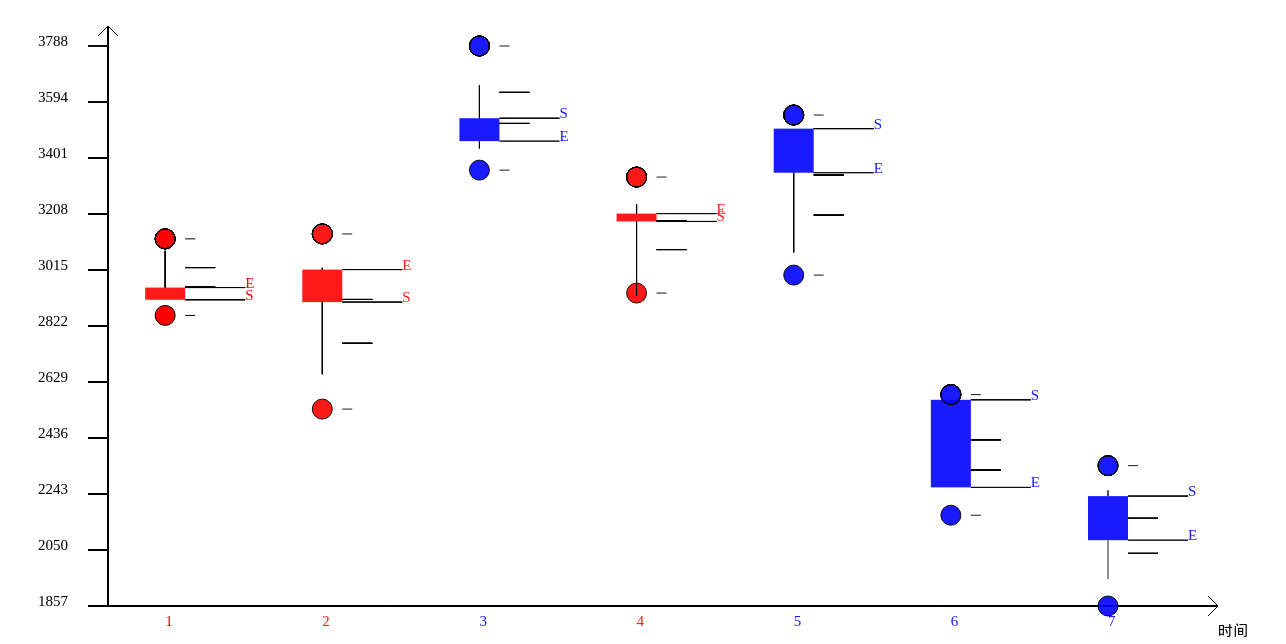
\includegraphics[scale=0.25]{./images/figure-4-1}
	\caption{时序输入数据}
	\label{Figure 4-1-1}
\end{figure}
























